% SVN info for this file
\svnidlong
{$HeadURL$}
{$LastChangedDate$}
{$LastChangedRevision$}
{$LastChangedBy$}

\chapter{Introduction}
\labelChapter{intro-chap}

\begin{introduction}
\end{introduction}

\section{Minimum Value Proposition}
\begin{introduction}
  
\end{introduction}
\subsection{Overview of the Frienso UI}
\begin{figure}
 \centering
  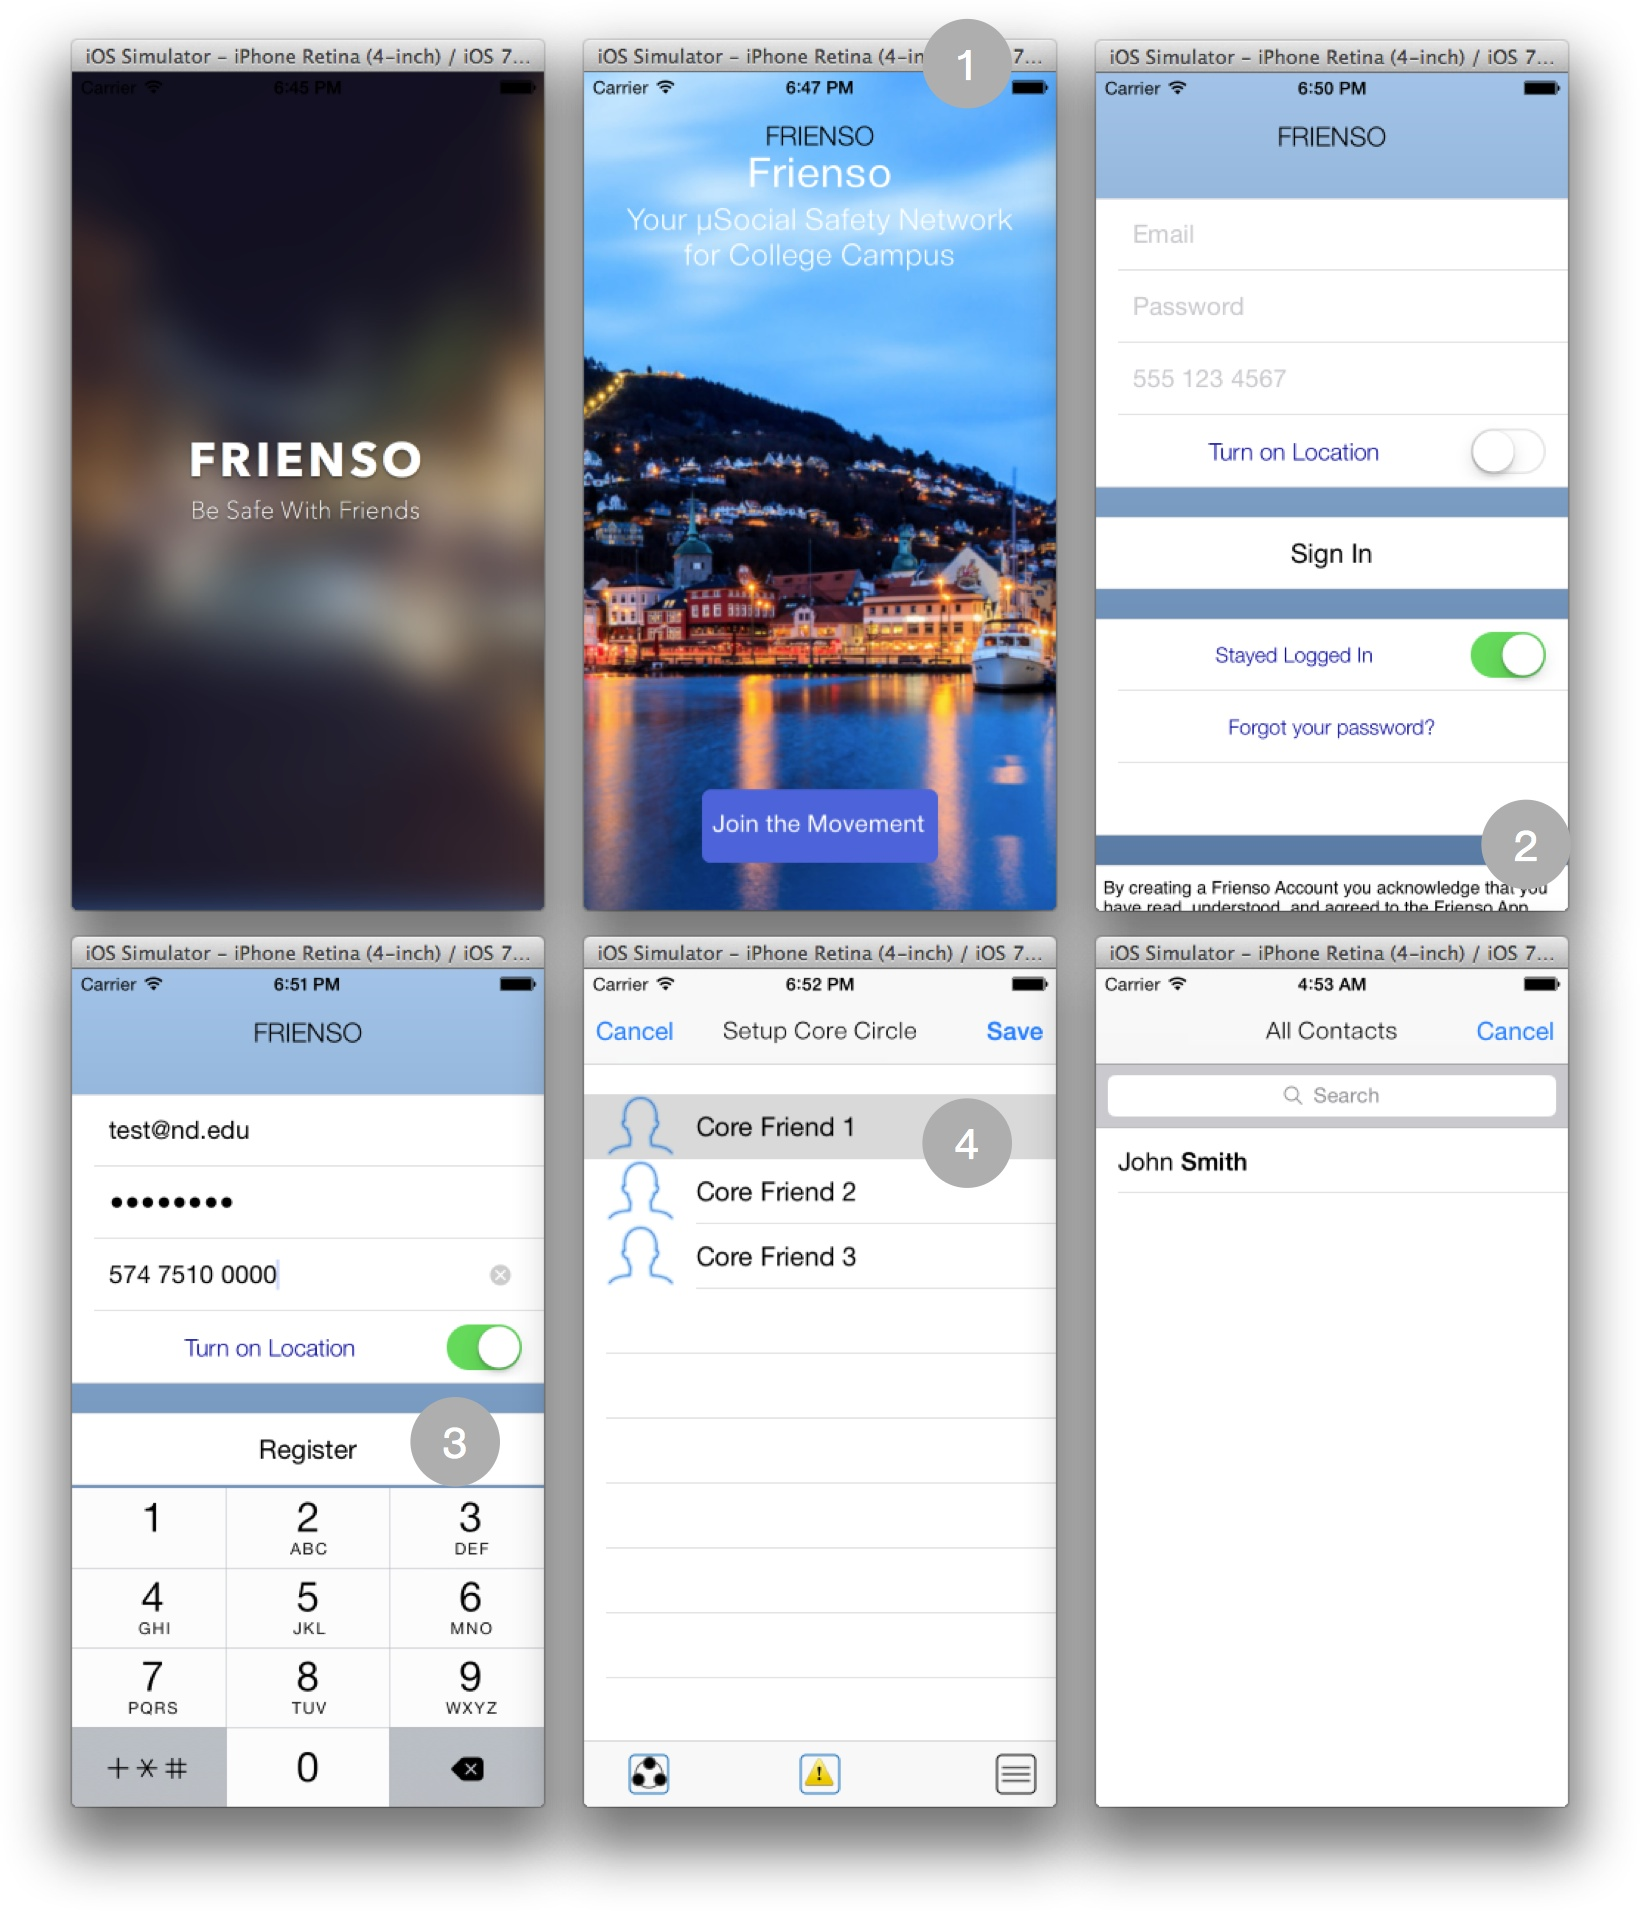
\includegraphics[width=\textwidth]{images/mvp_actual0.jpg}
	\caption{
	Login or registration   
	}
	% \label{fig:UEGraph}
	\end{figure}

\begin{figure}
 \centering
   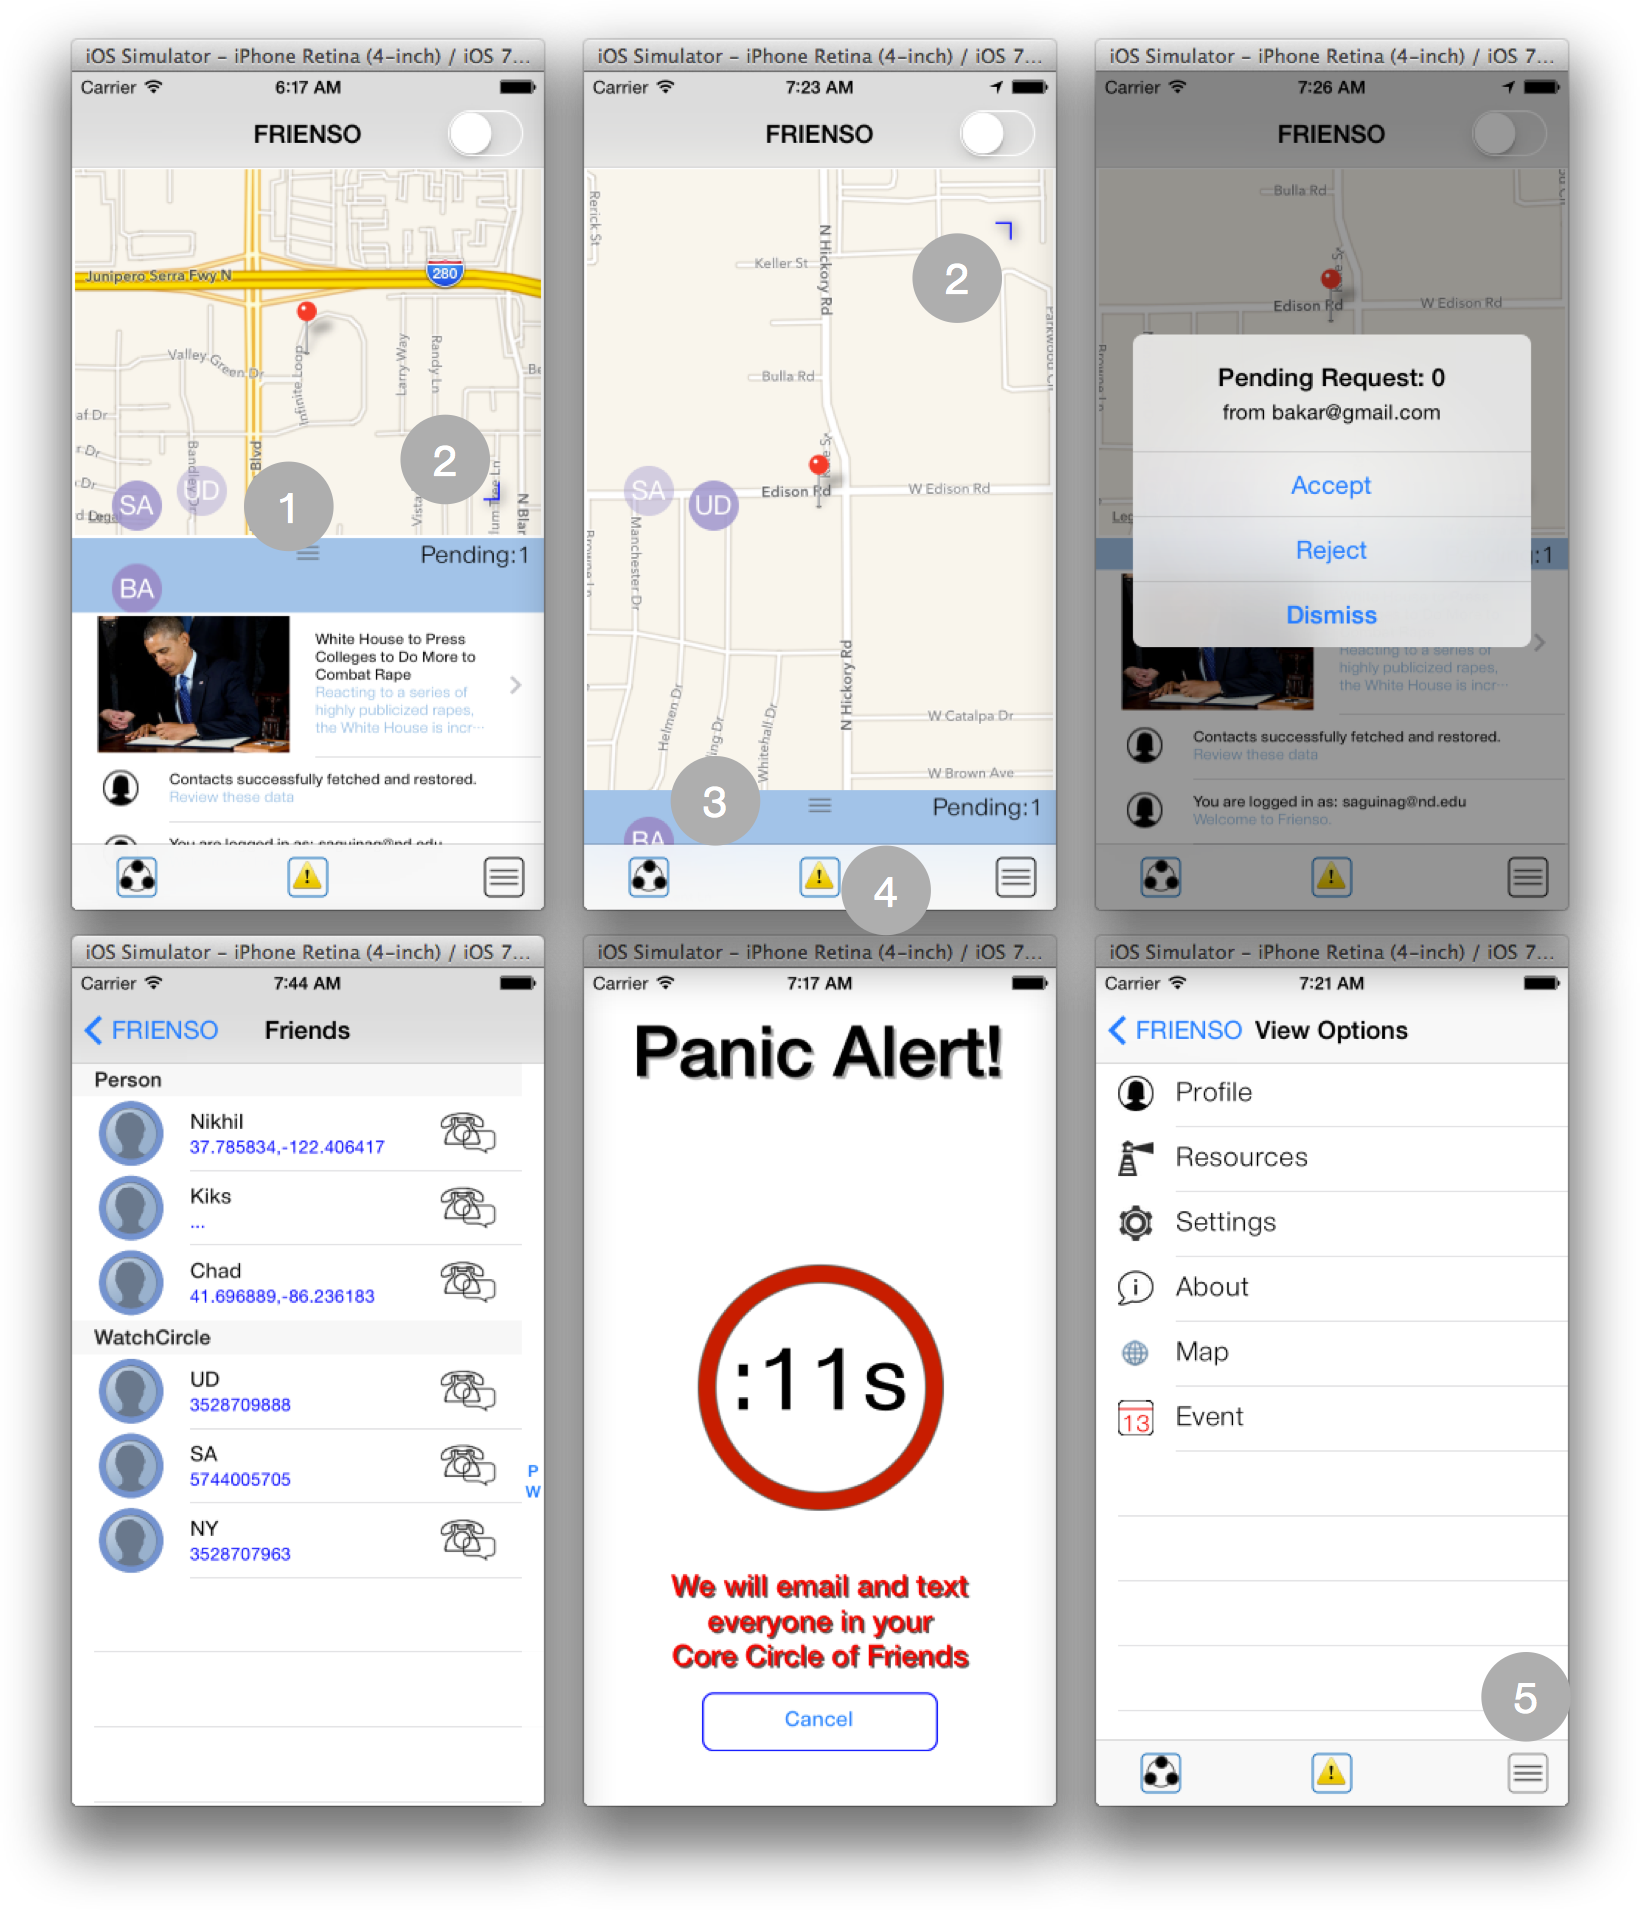
\includegraphics[width=\textwidth]{images/mvp_actual1.png}
    \caption{
	Home view and toolbar features: Home view, Fullscren mapview, Pending requests drawer, 
	Friends view, HelpNow view, View options (top left to bottom right).
%	\raisebox{.5pt}{\textcircled{\raisebox{-.9pt} {\small{8}}}} something
	}
	% \label{fig:UEGraph}
	\end{figure}
\subsection{CoreFriends Network Creation}


\section{Team Collaboration}
\subsection{README iOS Code File}
The iOS project folder contains the file \texttt{README.md} to be used to maintain brief
descriptions of the app's version and build number.  The build number is a number 
generated from the git commits. The build version number is updated each time a new 
executable is generated for ad-hoc distribution.

In addition to the app's version, the README file maintains a list of TODO items and 
descriptions of how they were completed.


\subsection{Team Collaboration on Github}
\href{https://help.github.com/articles/resolving-merge-conflicts}{\color{blue}{Resolving merge conflicts}}
\section{Documenation Structure}
%\lettrine[nindent=-3pt]{P}{raesent fermentum tristique} nunc, a rutrum ligula

%\section{Flow Chart}

\section{Features}

\subsection{Pending Requests}
  Pending requests fall into four types: watch, helpNow, and coreFriend.
  Users have the following options: to accept, reject, or dismiss the request.
  
  
  
\subsubsection{Type: watch}
  Requests of type \emph{watch} are accessed when a user that added you to their 
  coreFriends circle has initiated a 'watchMe' alert.
  
  \textbf{watch} alerts will share your location in near real time only with those
  in your coreCircle and only if they have accepted your 'watch' requests.  Accept or 
  reject allows for a feedback mechanism.  Users that initiate a watchMe request will
  know who is watching them for the duration of the watchMe alert active period.
  
\subsubsection{Type: helpNow}
  Requests of type \emph{helpNow} are accessed when a user has initiated an urgent help
  request.  Initiating this request type triggers SMS texts to go to those in
  one's coreFriends circle (aka coreCircle) and push notifications.
  
  \textbf{helpNow} alerts will share your location in near real time only with those
  in your coreCircle regardless if they've accepted your request.  Users that initiate 
  a helpNow request will also be prompted to dial campus police or 911 automatically.
   
\subsubsection{Type: coreFriend }
  Requests of type \emph{coreFriend} are accessed when i) a user creates its $\mu$social
  network.  The user selects from it's contacts up to three friends, and ii) when the user
  changes or edits it's coreCircle.  The actions after the user hits 'save' are to update
  the local data-store (NSUserDefaults, and CoreData) and update the cloud-store (Parse).
  
  \noindent \textbf{coreFriend} requests notify contacts that they have been chosen to be 
  a trusted friend on the Frienso app.  The notification will appears on their phone's 
  Frienso app or as a SMS text.  
  
  These requests have bidirectional properties, you might ask user X to be in your 
  coreCircle and that same user might ask you to be in their coreCircle.  In this case,
  the user should only appear once in your Frienso friends list.
  
%  Requests of type \emph{watchFriend} are requests by others (including those in your 
%  coreCircle) to include you in their coreCircle.  This indicates you are a trusted
%  Friend to be used in the Frienso app to help in cases of 'watch' or 'helpNow' alerts.
%  
%  \textbf{watchFriend} requests will not duplicate data on any user's phone. If the 
%  person requesting to add you to their coreCircle is also a person in your coreCircle
%  the name shall appear only once.  Future versions of the app will visually note 
%  the two-way relationship.       
  
\section{Data-Store Structures}
\subsection{NSUserDefaults}
Key-value standard defaults:
	\begin{table}[ht!]%
	%\caption{Table caption \label{tab:table_label}}
	\begin{tabularx}{\linewidth}{ l X }
	\emph{Key} & Value \\\hline
	\emph{adminID} & username, email \\
	\emph{adminPass} & password \\
	\emph{userName} & user's email \\
	\emph{userEmail} & user's email \\
	\emph{adminInParse} & flag, 0 = Not in parse\\
	\emph{userPhone} & user's phone number \\
	\emph{CoreFriendsContactInfoDicKey} & NSDictionary of user's coreCircle\\
	\end{tabularx}
	\end{table}%
\subsection{CoreData}
The Frienso projects has the following NSManagedObject subclass files and entity 
attributes:
\begin{itemize}
\item \texttt{CoreFriends[.h,.m]}
	\subitem \small{\@property (nonatomic, retain) NSString * coreEmail;}
	\subitem \small{\@property (nonatomic, retain) NSString * coreFirstName;}
	\subitem \small{\@property (nonatomic, retain) NSString * coreLastName;}
	\subitem \small{$\ldots$ see the CoreDataFiles for more details}
\item \texttt{FrienEvent[.h,.m]}
	\subitem \small{\@property (nonatomic, retain) NSString * eventTitle;}
	\subitem \small{\@property (nonatomic, retain) NSString * eventSubtitle;}
	\subitem \small{\@property (nonatomic, retain) NSString * eventObjId;}
	\subitem \small{$\ldots$ see the CoreDataFiles for more details}
\item \texttt{FriensoEvent[.h,.m]}
	\subitem \small{\@property (nonatomic, retain) NSString * resTitle;}
	\subitem \small{\@property (nonatomic, retain) NSString * resDetail;}
	\subitem \small{\@property (nonatomic, retain) NSString * resUrlLink;}
	\subitem \small{$\ldots$ see the CoreDataFiles for more details}\normalsize
\end{itemize}

\subsection{Parse - Cloud Store}
This projects uses Parse as the cloud-store back-end and can accessed at here: 
\href{https://www.parse.com/apps/frienso--2/collections}{$\leadsto$ Parse/Dashboard/Data Browser 
link}.

\begin{table}[ht!]%
	\caption{Parse Frienso Classes \label{tab:table_label}}
	\begin{tabularx}{\linewidth}{ l X }
	\textbf{Classes} & \textbf{Description} \\\hline
	\emph{User}  & The standard user object \\
	\emph{UserCoreFriends}  & Dictionary data structure holds each user's coreCircle \\
	\emph{Resources}        & College/University resources \\
	\emph{UserConnections}	& Linking a phone number to a user (class to be deprecated,
	because the phone number has been added to the User class).\\
	\emph{CoreFriendRequest}& $\dagger$\\
	\emph{TrackRequest} 	& $\dagger$\\
	\emph{UserEvent} 		& $\dagger$\\
	\end{tabularx}\end{table}%

\noindent \textbf{$\dagger$} these classes are under construction.



